\documentclass[12pt]{article}
   
   \usepackage[utf8]{inputenc}
   \usepackage{graphicx}
   \usepackage{float}
   \usepackage{subcaption}
   \usepackage{mathtools}
   \usepackage{amsmath}
   \usepackage{amsfonts}

   \addtolength{\hoffset}{-0.7in}
   \addtolength{\textheight}{1.5in}
   \addtolength{\textwidth}{1.5in}
   \addtolength{\voffset}{-1in}
 
\title{EE 234: Experiment - 1 \\
       Power Analysis in balanced 3 phase circuits}
       
\author{Chaitanya gardas, 180070021  \
Karthik gvb, 180070022 \\
Hitesh kandala, 180070023}
\date{January 27, 2020}
%________________________________________________________________________________________________
\begin{document}

  \maketitle
  
  \section{Aim of the experiment}
  
  This experiment is devoted to the power measurement in a balanced three phase circuit for STAR load, DELTA load and also the improvement of power factor specifically for an induction motor.
  
  %_______________________________________________________________________________________
  
  \section{Overview of the experiment}
  The Experiment is mostly connecting many wires carefully and noting the observations. 
  \begin{itemize}
      \item In the first part of the experiment, we measured line-line voltages and line-line currents as well as their corresponding power and power factors using two power analysers for STAR load and DELTA load
      
      \begin{figure}[H]
          \centering
          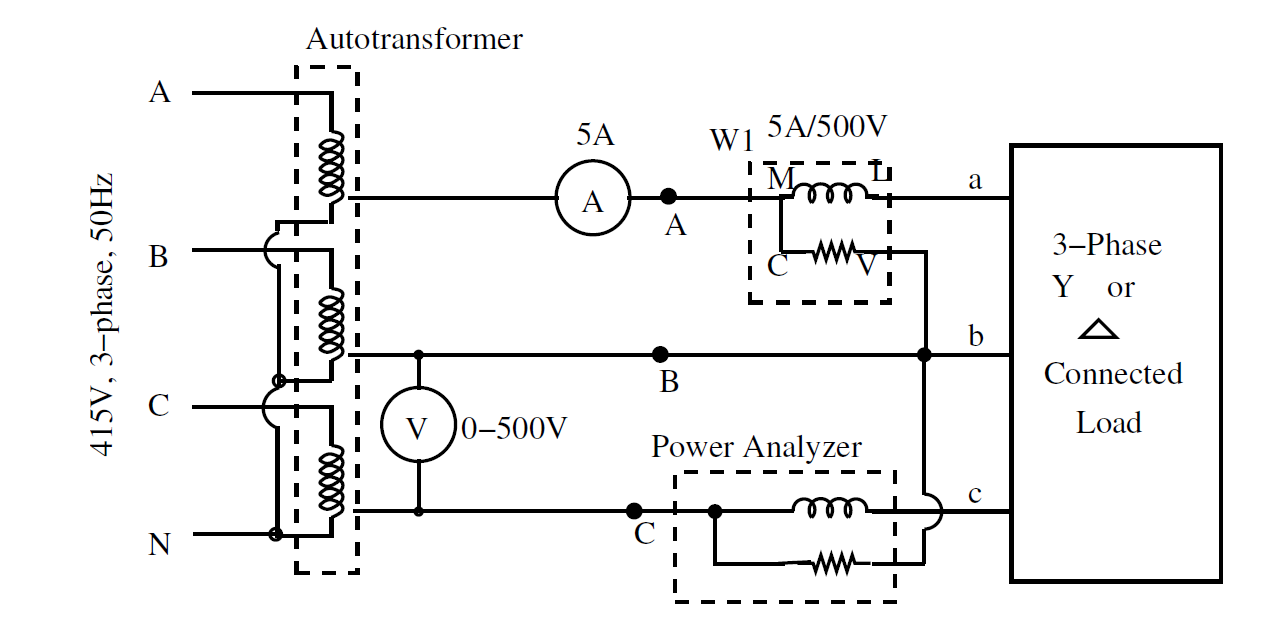
\includegraphics[width = 0.9\linewidth]{LAB-1/1.PNG}
          \caption{Circuit Diagram to measure power consumed by 3-phase Load 
           using 2-Wattmeters}
      \end{figure}
      
      \begin{figure}[H]
          \centering
          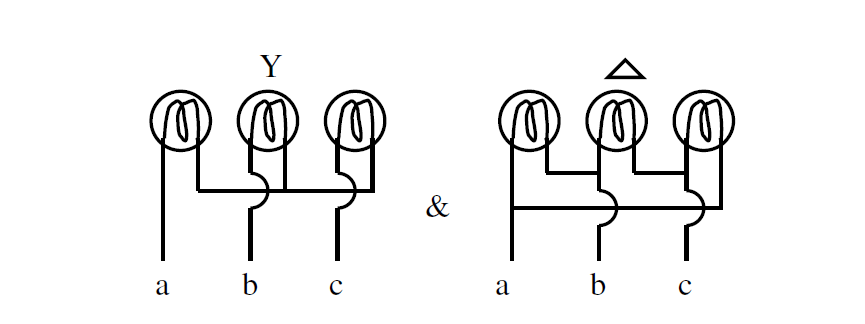
\includegraphics[width = 0.7\linewidth]{LAB-1/1-1.PNG}
          \caption{3-Phase Load connection: Star & Delta}
      \end{figure}
      
      The top power analyser measures $\bar{V}_{ab}$ and $\bar{I}_{A}$ and the bottom analyser measures $\bar{V}_{cb}$ and $\bar{I}_{C}$ hence their power measurements would be,
      
      \begin{equation}
         \ \ \ W_1 = V_{ab}I_{A}cos\angle(\bar{I}_{A} \ \& \ \bar{V}_{ab}) \ \ \ and \ \ \ W_2 = V_{cb}I_{C}cos\angle( \bar{I}_{C} \ \& \ \bar{V}_{cb}) 
      \end{equation}
      
      Phase difference between $\bar{V}_{ab}$ \& $\bar{I}_{A}$ is $(30 + \theta)$ and $\bar{V}_{cb}$ \& $\bar{I}_{C}$ is $(\theta - 30)$ from the relations between line voltages and phase voltages hence
      
      \begin{align}
          \ \ \ W_1 = V_{L}I_{L}cos(30 + \theta) \ \ \ &and \ \ \ W_2 = V_{L}I_{L}cos(\theta - 30) \\
          W_1 + W_2 = \sqrt{3}V_{L}I_{L}cos\theta &\implies total \ power \ of \ 3 \ phase \ load
      \end{align}
      
      \item 
      
      \begin{figure}[H]
          \centering
          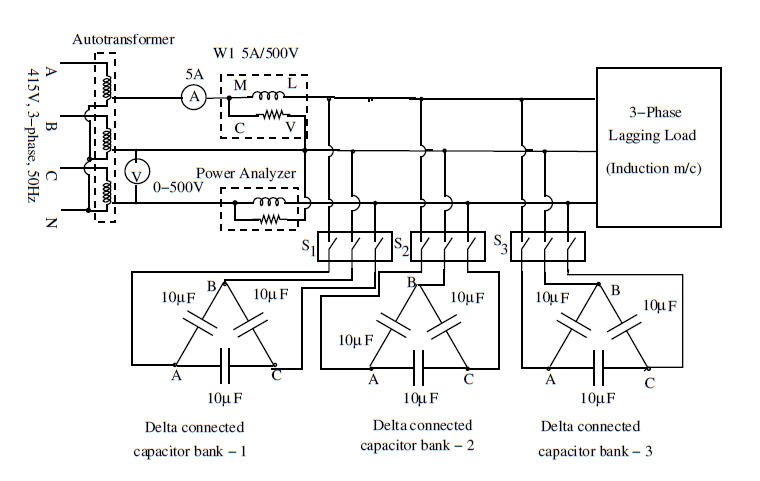
\includegraphics[width = 0.9\linewidth]{LAB-1/2.PNG}
          \caption{Circuit diagram for Power factor improvement}
      \end{figure}
      
      The last part was power factor improvement of an induction motor, we analysed the changes in power factor on connecting different number of identical capacitive delta loads to the induction motor, again with the same power analysers.
      
      \end{itemize}
  
  %_____________________________________________________________________________________________________
  
  \section{Observations}
  
      \subsection{Part-\rom{1} Star Connected Load}
      
          \begin{table}[H]
              \centering
              \begin{tabular}{|c|c|c|c|c|}
              \hline
                  Wattmeter & Voltage(V) & Current(mA) & Power(watts) & Power Factor \\
              \hline
              W1 & 386.3 & 426.8 & 142.5 & 0.865 \\
              W2 & 387 & 427.1 & 142.5 & 0.862 \\
              \hline
              \end{tabular}
              \caption{Wattmeter readings of Star connected load}
          \end{table}

      \subsection{Part-\rom{2} Delta Connected Load}
      
          \begin{table}[H]
              \centering
              \begin{tabular}{|c|c|c|c|c|}
              \hline
                   Wattmeter & Voltage(V) & Current(mA) & Power(watts) & Power Factor \\
              \hline
              W1 & 216.6 & 725.4 & 137.1 & 0.868 \\
              W2 & 216.4 & 724.6 & 135.55 & 0.863 \\
              \hline
              \end{tabular}
              \caption{Wattmeter readings of Delta connected load}
              \label{tab:my_label}
          \end{table}
          
        \subsection{Part-\rom{3} Power Factor improvement}
    
            \begin{table}[H]
                \centering
                \begin{tabular}{|c|c|c|c|c|c|}
                \hline
                Capacitance & Wattmeter & Voltage(V) & Current(A) & Power(W) & Power factor \\
                \hline
                \multirow{Without capacitance} & W1 & 216.2 & 2.71 & -199.88 & 0.343 \\ \cline{2-6}   & W2 & 215.9 & 2.740 & 364.8 & 0.614 \\ \hline
                \multirow{1 Bank} & W1 & 217.2 & 1.593 & -74.03 & 0.217 \\ \cline{2-6} & W2 & 216.4 & 1.598 & 241.3 & 0.698 \\ \hline
                \multirow{2 Banks} & W1 & 217.1 & 1.420 & -49.41 & 0.170 \\ \cline{2-6} & W2 & 216.9 & 1.083 & 214 & 0.913 \\ \hline
                \multirow{3 Banks} & W1 & 216.5 & 0.677 & 82.92 & 0.570 \\ \cline{2-6} & W2 & 216.1 & 1.466 & 82.20 & 0.325 \\ \hline
                \end{tabular}
                \caption{Wattmeter readings of induction motor with varying capacitance }
                \label{tab:my_label}
            \end{table}
       
       \begin{figure}[H]
       
          \begin{subfigure}{0.3\linewidth}
               \centering
               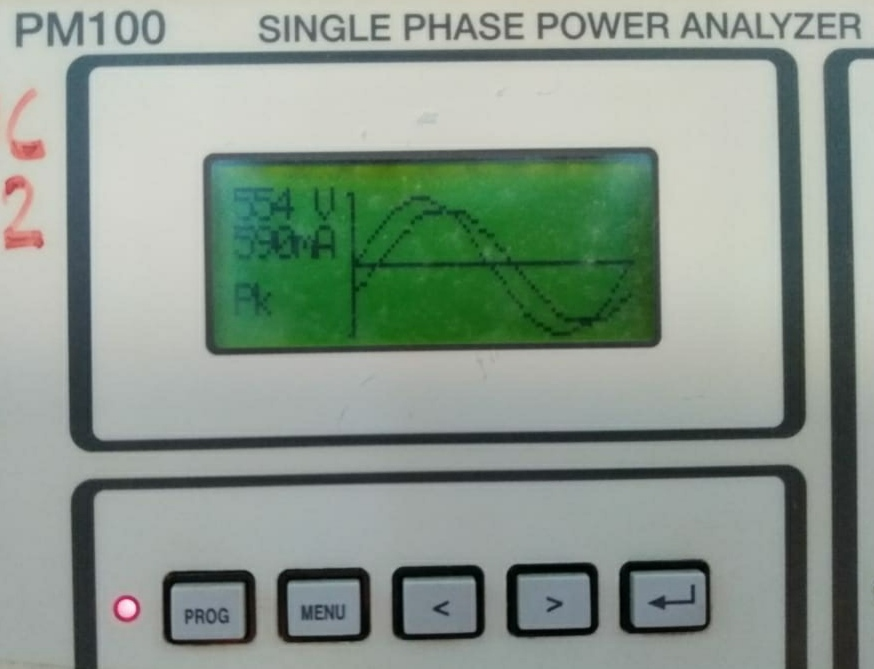
\includegraphics[width = \linewidth]{LAB-1/star.jpeg}
               \caption{For Star Load}
          \end{subfigure}
          \begin{subfigure}{0.3\linewidth}
               \centering
               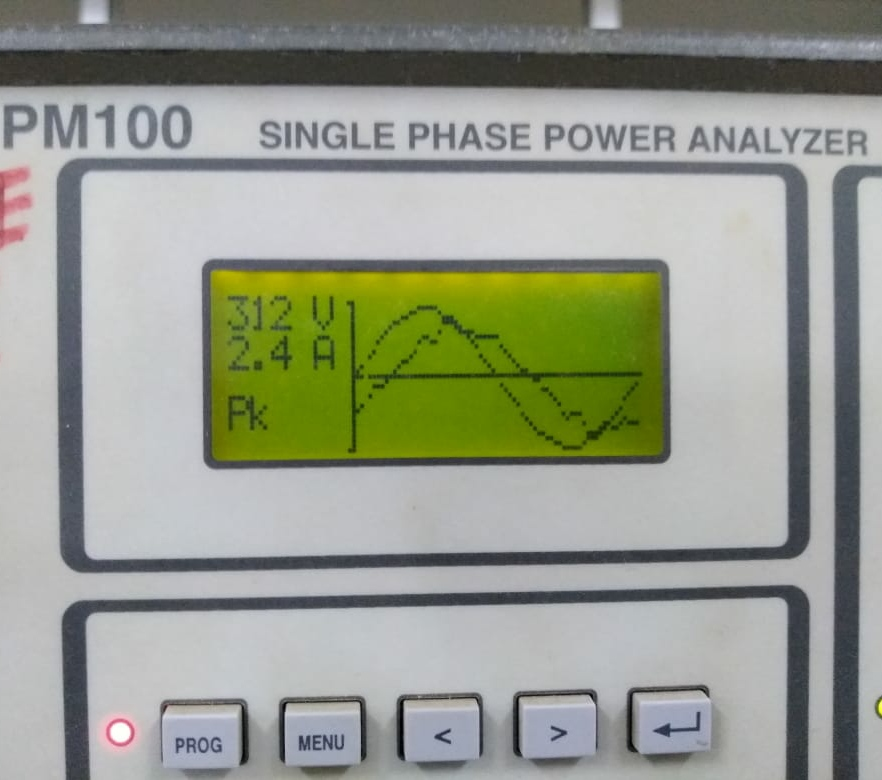
\includegraphics[width = 0.85\linewidth]{LAB-1/2 bank.jpeg}
               \caption{With 2 banks connected}
          \end{subfigure} 
          \begin{subfigure}{0.3\linewidth}
               \centering
               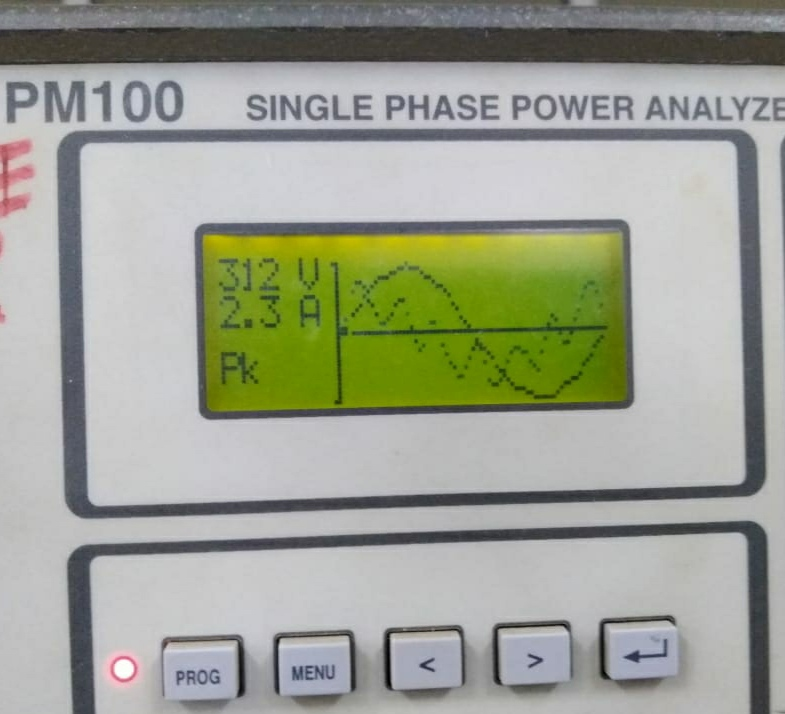
\includegraphics[width = 0.85\linewidth]{LAB-1/3 bank.jpeg}
               \caption{With 3 banks connected}
          \end{subfigure} 
          \caption{Waveforms of line-Voltage and line-current}
       \end{figure}
       
       
    
    %____________________________________________________________________________________________________
    
  \section{Conclusion}
  
    \begin{itemize}
        \item From the equations-(2), (3) we can find out the power factor which is given by: 
        \begin{equation}
            cos\theta = cos\left[tan^{-1}\left(\sqrt{3}\frac{W_1 - W_2}{W_1 + W_2}\right)\right] 
        \end{equation}
        
            \begin{table}[H]
                \centering
                \begin{tabular}{|c|c|c|}
                    \hline
                    Load & Total Power & Power factor  \\ \hline
                    Star & 285.0 & 1 \\ \hline
                    Delta & 272.65 & 0.99 \\ \hline
                \end{tabular}
                \caption{Part-1 \& Part-2}
            \end{table}
            
            \begin{table}[H]
                \centering
                \begin{tabular}{|c|c|c|}
                    \hline
                    Load & Total Power & Power factor  \\ \hline
                    Without capacitance  & 164.92 & 0.1663 \\ \hline
                    1 Bank & 167.27 & 0.293 \\ \hline
                    2 Bank & 164.59 & 0.3393 \\ \hline
                    3 Bank & 165.12 & 0.99 \\ \hline
                \end{tabular}
                \caption{Part-3}
            \end{table}
        \item In Part-1 and Part-2 the Load is purely resistive hence the power factors are nearly 1.
        \item We can identify that the power factor increased as the number of capacitor loads increased which implies that the added capacitor loads are being compensating the inductive behaviour of induction motor.
        \item We can also identify that with all three capacitor banks connected the power factor reading of 1st wattmeter is larger than the 2nd wattmeter which implies that the actual load power factor is leading.
        \item In Part-3 the load is inductive untill all the capacitor loads are connected i.e power factor is lagging till 2 bank connection and with all three capacitor banks connected the power factor changes to leading.
        
    \end{itemize}
  
  \newpage
  
  %_______________________________________________________________________________________________________
  
  \section{Questions to be answered}
  
  \begin{itemize}
      \item A. With all three capacitor banks connected across the load, the source powerfactor might be now leading. How can you infer this from the readings? Are there any advantages of overcompensating the load?\vspace{0.2cm} \\
      \textbf{Ans} One of the two wattmeters show an increase in powerfactor readings till 2 capacitor load connection and then a decrease in power factor as soon as the third capacitor load is connected where as the other wattmeter powerfactor reading first decreased and then increased, this implies that the source powerfactor has changed from lagging to leading by connecting the third load. Overcompensation is mostly non-advantageous as it doesn't provide high powerfactor.    
      \item B. You might have observed the voltage \& current waveforms on the power analyzer (step-iv in `section 4.1'). Why is the angle between these two waveforms is $30^o$ even though the load is purely resistive? \vspace{0.2cm} \\
      \textbf{Ans} The waveforms are of line-line voltage and line-line current, hence even the impedance is resistive there exists a phase difference of $30^o$ between observed current and voltage waveforms.
      \item C. What is the reason for reducing the voltage to zero every time before switching on the capacitors?\vspace{0.2cm} \\
      \textbf{Ans} The circuit is working with AC signals, hence if voltage is not reduced to zero before switching on the capacitors then the initial conditions in the passive elements aren't zero which then interfere and cause improper/undesired observations. 
      \item D. You have been given thick and thin wires for connections. Which one will you use for connecting (i) an ammeter and (ii) a voltmeter? Justify your answer.\vspace{0.2cm} \\
      \textbf{Ans} We would use the thick wire for connecting an ammeter and the thin wire for connecting a voltmeter.\vspace{0.2cm}\\
      Ammeter is connected in series to find current hence it's resistance should very low(and $Resistance \propto \frac{1}{Area}$) and a voltmeter is0 connected in parallel to find voltage hence should not allow current which implies a large resistance which is not offered by a thick wire.
      \item E. During the late hours of the night you might have observed the intensity of the incandescent bulb is much higher compared to that during 7-8pm. What could be the reason?\vspace{0.2cm} \\
      \textbf{Ans} The reason might be that as the total load increase power acquired by each load decrease,  During the late hours of the night the total power consumption is less compared to that of during 7-8pm, hence bulb during late night acquires relatively more power and glows with higher intensity
      \item F. Why do the single phase motor driven appliances experience vibration? \vspace{0.2cm} \\
      \textbf{Ans} A single phase supply offers time varying power to the load, hence the single phase motor experiences a rise and fall in it's mechanical power obtained from the time varying electrical power supplied by a single phase source. This rise and fall in motor's mechanical power causes it to vibrate. 
      \item G. You might have observed the power sockets with two pins while, some of them with three pins. What is the difference between these power sockets?\vspace{0.2cm} \\
      \textbf{Ans} The difference is the Earthing pin in three pin sockets, 2 pin sockets just have the phase and neutral where as the three pin sockets have phase and neutral along with earth(To avoid shocks to liable elements).
      \item H. Utilities use energy meters to measure the energy consumed by consumers. Energy is given by
      \begin{align}
          E &= \int P dt \\
          E &= \int (VIcos\theta) dt
      \end{align}
      where P is the power consumed by the load. From Fig. 1 it can be inferred that though the consumer is drawing `I' A of current, he/she is being charged only for $I cos\theta$. In other words there is no apparent advantage of improving the power factor to unity. Is this correct? Justify your answer.\vspace{0.2cm} \\
      \textbf{Ans} No. As we know, only average power is the actual useful power used by the utilities. But still, all the electrical equipment have to be designed in such a way to handle both current and voltage magnitudes. Hence, a large reactive power may lead to unwanted cost bearing on equipment and their repairs. 
      
      And also, decrease in power factor leads to increase in magnitude of current flowing through the lines, for the same amount real power. Due to high currents their are high transmission losses($I^2R$), and a voltage drop at the load decreasing the efficiency. So, it is all efficient to keep the power factor close to 1. 
      \item I. Suppose (3+j4)  kVA load is being supplied at $230 V$ ( load voltage) and the transmission line has an impedance of $(1 + j1)\Omega$. Determine the following: \\
      (a) voltage at the source terminals \\
      (b) power loss in the transmission line \\
      (c) the required kVAR rating of the capacitor to compensate the load fully (source supplies only the active component of current). \\
      (d) source current, drop is the transmission line, power loss in the transmission line after compensation.\vspace{0.2cm} \\
      \textbf{Ans}
      \begin{align}
          S = \bar{V} \bar{I}^* \implies |\bar{I}| &= \frac{|S|}{|\bar{V}|} = \frac{5K}{230} = 21.74 \ A \\
          S = \bar{V} \bar{I}^* \implies S &= \bar{V} \frac{\bar{V}^*}{Z^*} \implies Z = \frac{|\bar{V}|^2}{S^*} \vspace{0.3cm}\\
          Z = \frac{(230)^2 \times 10^{-3}}{3-4j} &= 6.348 + 8.464j \rightarrow Load \ impedance \\
      \end{align}
      (a)
      \begin{align}
       Source \ Voltage \ \bar{V} = &\bar{I}*total \ impedance \implies |\bar{V}| = |\bar{I}||Z| \\
       \bar{V} = 21.74 \times &(|6.348 + 8.464j + 1 + j|) = 260.5 V
      \end{align}
      (b)
      \begin{equation}
          power \ loss = |\bar{I}|^2 * Z = (21.74)^2 \times (1 + j) = 668.4\angle 45^o \ VA
      \end{equation}
      The average power loss i.e real power loss is $472.6 W$ \\
      (c) The reactive power of the load is 4kVAr, and transmission lines is 472.63. Hence to compensate it, we need a capacitor load of 4,472.63VAr(Leading load).\\
      (d)After compensating 
      
      Source current=Active current = $I\cos(\theta)$=13.04A\\
      Drop in the transmission line= $13.04(1+j)=13.04+j13.04$\\ 
      Power loss in transmission line = $I^2R=(13.04)^2.1=170.04W$
      \item J. Find the per phase capacitance necessary to improve the powerfactor to unity in Part-III ( section-iv) for the following capacitor connections:\\
      i. Star \\
      ii. Delta\vspace{0.2cm} \\
      \textbf{Ans} To improve the factor to unity, a capacitor bank must be connected in parallel to the load. In part-$\rom{3}$, the observed values of line voltage and current for delta connected motor load are $V_L=216.05$, $I_L=2.725A$ and power factor= 0.1663.
      Therefore, for star connected ,$$I_C=I_{Load}\sin(\theta)\Rightarrow C=\frac{\sin(\theta
      )I_L}{V_{phase}\omega}=68.6\mu F$$
      For delta, phase capacitance $C_{delta}=C_{star}/3=22.86\mu F$
  \end{itemize}
\end{document} 